\chapter{Arquitectura Final}
\label{cap:ArquitecturaFinal}


Se adjunta la Figura~\ref{fig:workflow_v5} con el objetivo de facilitar la comprensión del modelo 
del Prototipo 5. El trabajo queda dividido en 5 fases: generación de audio, conversión a tensores, 
preparación del dataset, entrenamiento (con múltiples opciones de arquitectura) e inferencia paramétrica.
\begin{figure} 
    \centering
    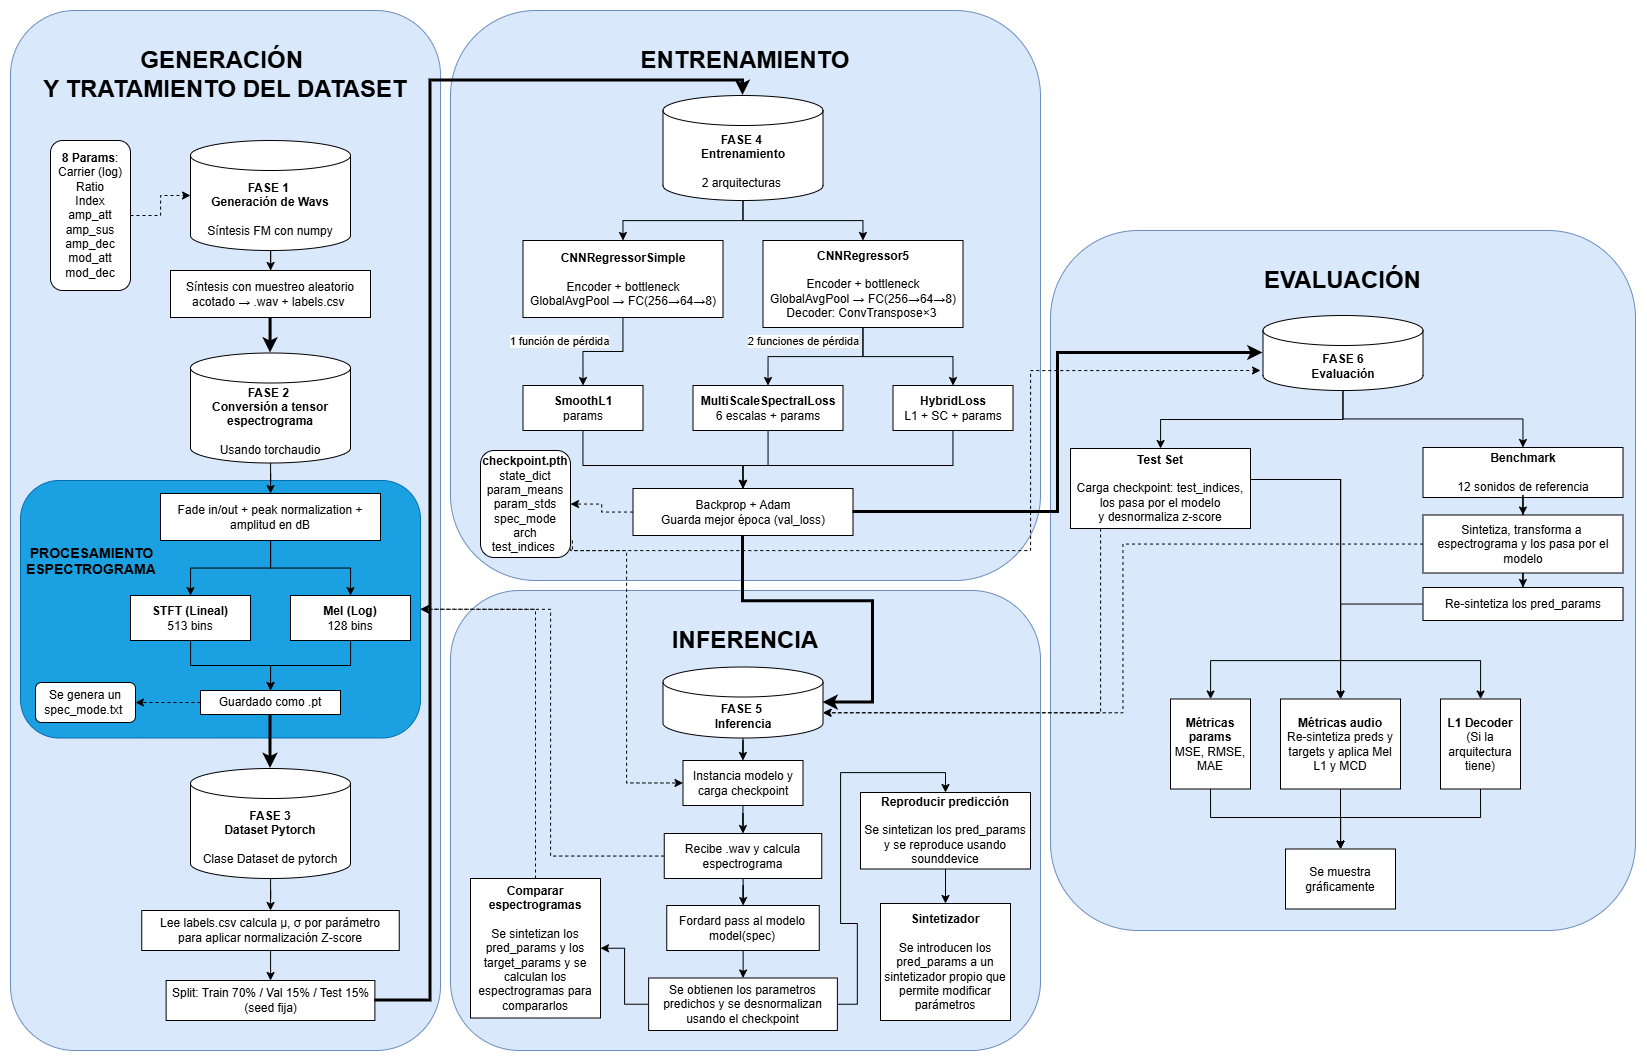
\includegraphics[width=1\textwidth]{Imagenes/Bitmap/diagrama}
    \caption{Flujo de trabajo del Prototipo 5: desde la síntesis matemática hasta la inferencia y evaluación del modelo.}
    \label{fig:workflow_v5}
\end{figure}
\section{Expansión Paramétrica: Evolventes y Generación Aleatoria del Dataset}
Las predicciones del \textbf{Prototipo 4} consiguen replicar detalladamente el timbre. Sin embargo,
los sonidos generados en esta etapa están muy alejados de las aplicaciones reales del \textbf{Sound Matching}. 
Por esta razón, se propone un nuevo modelo en el que se explora ampliar
la dimensionalidad de 3 a 8 parámetros. A las variables
fundamentales (frecuencia portadora, ratio e índice), se le añaden las envolventes temporales: 
la envolvente de amplitud (\textit{attack, decay} y \textit{sustain}) y la envolvente del índice de 
modulación (\textit{attack} y \textit{decay}).

Son precisamente estas características del \textbf{Prototipo 5}, por las que es necesario una nueva 
forma de generación del dataset. La ampliación de 3 a 8 parámetros hace computacional inviable generar
el dataset mediante un barrido de combinaciones posibles. Para dar solución a esta limitación, se genera el dataset
por muestreo aleatorio. 

El sistema genera un número (N) de muestras de audio con valores continuos aleatorios,
en base a unos rangos de valores específicos para cada parámetro. Para cada uno de ellos 
se utiliza una distribución uniforme, a excepción de la frecuencia portadora (\textit{Carrier}) que 
se realiza en escala logarítmica. De esta forma se simula la percepción humana del sonido. 

En primer lugar, se sintetizan los N archivos \textit{.wav} mediante la librería \textbf{NumPy} y la formulación matemática de la FM (Fase 1). 
Se define una frecuencia de muestreo (\textit{sample rate}) de 44100 Hz
y se incrementa el tiempo de duración de 1 a 2 segundos, con el fin de asegurar un margen temporal
necesario para analizar y percibir las variaciones en el sonido provocadas por las envolventes. 
Estas envolventes se generan sobre un vector de tiempo unificado. 

En la Fase 2, los audios generados \textit{.wav} se convierten a tensores nativos de \textit{PyTorch}. Se cargan mediante \textit{torchaudio} y
se les aplica un suavizado de amplitud en los extremos (\textit{fade-in} y \textit{fade-out}) con el objetivo de 
evitar chasquidos o ruidos indeseados. Tras una normalización de pico, se aplican las dos transformaciones principales:
de audio a espectrograma y de amplitud lineal a logarítmica (dB). Para la representación acustica, el programa permite elegir
entre dos métodos, con el fin de llevar a cabo diferentes pruebas de experimentación. Por un lado, se encuentran 
los espectrogramas en formato lineal, mediante \textbf{STFT} con 513  \textit{bins}\footnote{El término \textit{bin} hace referencia los intervalos de la Tranformada de Fourier (FFT). 
El tamaño de ventana utilizado para la creación de los espectrogramas es de 1024 ($N_{fft} = 1024$), lo que genera
$1024 / 2 + 1 = 513$ intervalos o \textit{bins} de frecuencias}de frecuencia. Y por el otro lado, 
se da lugar a elegir un formato logarítmico-perceptual (\textbf{Mel} con 128 bandas), el cual tiene un mayor potencial para
la representación del sonido de manera similar a la percibida por el humano. Posteriormente, se extrae
la magnitud de la señal, se convierte a decibelios (dB) y se guarda como tensores (formato \textit{.pt}). Además,
se genera un archivo (spec\_mode.txt) que indica el tipo de espectrograma utilizado.

Para terminar con el tratamiento del dataset, se estructuran los tensores en una clase Dataset de PyTorch
(\textit{SpectrogramTensorDataset}). Se lee el registro de etiquetas (\textit{labels.cvs}), el cual contiene todos los
valores de los parámetros de cada audio, y se calcula la media y desviación estándar global de cada uno de ellos. Con estas estadísticas
se aplica una normalización de puntuación estándar (\textit{Z-score}), nivelando así las diferencias entre las escalas
de los parámetros, consiguiendo igualar las importancias de cada uno en el cálculo del gradiente.
Finalmente, el dataset se divide, mediante una semilla fija, en: 70\% para entrenamiento, 15\% validación y se guarda otro 15\%
como conjunto de pruebas (\textit{Test set}).

La fase de entrenamiento se caracteriza por permitir la elección de diferentes arquitecturas y funciones de pérdida con el fin de experimentar. De esta 
forma, se pueden probar diferentes combinaciones para ver cual es más interesante en tiempo o precisión.
\begin{itemize}
 \item \textbf{Arquitecturas: }Se dispone de dos topologías convolucionales diferentes:
    \begin{itemize}
        \item \textbf{CNNRegressorSimple: }Está formada por un \textit{Encoder} de tres bloques convolucionales,
        un \textit{Bottleneck} y una cabeza de regresión pura (\textit{Global Average Pooling}). Esta última está conectadas
        a un Perceptrón Multicapa que acaba en 8 neuronas. A pesar de que la red ejecuta un entrenamiento rápido, al carecer de reconstrucción 
        no se garantiza que el \textit{Encoder} esté extrayendo de manera acertada la estructura del espectrograma, prediciendo únicamente números.
          
        \item \textbf{CNNRegressor5: }Se trata de una expansión del modelo anterior, incorporando una segunda cabeza de predicción. 
        Se añade un \textit{Decoder} que consta de 3 capas convoluvionales traspuestas, las cuales tratan de reconstruir el espectrograma 
        a partir del espacio latente. Así pues, esta etapa fuerza al \textit{Encoder} a capturar la riqueza temporal y tímbrica del sonido para evitar
        un error grande.
    \end{itemize}
 \item \textbf{Funciones de Pérdida: } Para el modelo simple, se evalua la diferencia paramétrica únicamente mediante
        \textbf{SmoothL1 Loss}. Esta se utiliza por su robustez y versatilidad en la regresión numérica: cuando la diferencia 
        entre el valor real y el predicho es muy pequeña, se comporta como un Error Cuadrático (L2), lo que suaviza la convergencia
        de gradientes; y ante desviaciones grandes, se asemeja al Error Absoluto (L1), de forma que los casos aislados que se alejan del resto 
        no desestabilicen la red. Esta función de pérdida tiene la desventaja de no tener en cuenta la no-inyectividad de la síntesis FM.

        En cuanto al modelo CNNRegressor5, se permite la elección de una de las siguientes funciones de pérdida:
    \begin{itemize}
        \item \textbf{HybridLoss: } % Es igual que la del prototipo anterior, quizá no la debería de explicar de nuevo
        Es una función de pérdida híbrida, que combina el Error Absoluto Medio (L1) de la reconstrucción del 
        espectrograma, un refuerzo estructural de Convegencia Espectral (SC), y la penalización paramétrica anterior.
        La primera se lleva el peso principal (de 1.0), calcula el Error Absoluto Medio píxel a píxel entre el espectrograma original y el reconstruido (en decibelios).
        La Convergencia Espectral (SC) se aplica con un peso medio (de 0.5) para evitar los espectros borrosos generados por L1. Esta métrica calcula la norma de Frobenius 
        para evaluar la energía global (relación armónica), regularizando el timbre. A la penalización paramétrica se le da una importancia muy baja (0.05), ya que no es demasiado importante
        debido al carácter no inyectivo de la síntesis FM.
          
        \item \textbf{MultiScaleSpectralLoss: } Esta función está inspirada en el modelo de síntesis diferencial DDSP. Al estar utilizando 
        espectrogramas, se simulan los distintos tamaños de ventana de Fourier mediante agrupamientos espaciales temporales (\textit{Average Pooling}).
        Se agrupa en seis factores (de 1, 2, 4, 8, 16 y 32) y se mide el error en cada una de esas escalas, siendo la media aritmética de esos errores
        el valor de pérdida total. El cálculo del error de cada escala primero se calcula la diferencia sobre las magnitudes
        lineales, la cual es útil para capturar picos de energía que pueden ser breves. A esto se le suma después la diferencia sobre las magnitudes en decibelios (logarítmico),
        multiplicada por un factor $\alpha$ de 1.0, por lo que se le está danto la misma relevancia que el error lineal, capturando así perfectamente
        la envolvente global y los momentos de baja energía. Mediante esta función, se consigue compara el sonido obtenido del original
        en varios niveles de resolución simultáneamente. Por último, se le suma el error paramétrico (\textit{SmoothL1}) con un peso muy bajo (0.05) con el objetivo
        de que la red no deje de tener mínimamente en cuenta los valores de los parámetros.   
    \end{itemize}
\end{itemize}
En la etapa final del entrenamiento, se encuentra el algoritmo de retropropagación (\textit{Backpropagation}), mediante el cual se actualizan
los pesos para así minimizar el error en la red, calculando los gradientes del error con respecto a cada nodo. 
Para la actualización de los pesos se emplea el optimizador \textbf{Adam} (\textit{Adaptive Moment Estimation}). Este se elige frente al descenso de gradiente común (SGD) debido al cálculo que hace 
de las tasas de aprendizaje adatativas e independientes para cada parámetro. A parte, se guardan los pesos de la época que ha conseguido 
el mínimo histórico con respecto al error sobre el conjunto de validación. Estos valores se almacenan en un archivo de punto de control (checkpoint.pth) junto
con el resto de información de contexto necesaria: 

\begin{itemize}
        \item \textbf{Parámetros de Desnormalización: } Contiene las medias y desviaciones estándar obtenidas en la Fase 3
        sobre los parámetros. Estas son necesarias para poder revertir el Z-score en las futuras predicciones. 
          
        \item \textbf{Contexto de Arquitectura: } Son las etiquetas que describen la topología (\textit{arch}: simple o full)
        y el tipo de espectrogramas (\textit{spec\_mode}: stft o mel) que se han utilizado para el modelo.
        
        \item \textbf{Aislamiento de Datos: } Contiene los índices del conjunto de prueba (\textit{test\_indices}), necesario para la evaluación.
        

\end{itemize}

La fase 5 consiste en la inferencia de parámetros de síntesis FM, mediante el modelo entrenado previamente, a partir
de audios. 

Al inicio de esta fase, se instancia el modelo y carga el punto de control, que instancia automáticamente
el tipo de red. 

La inferencia comienza cuando se recibe un archivo de audio (\textit{.wav}). En ese momento, se sigue el mismo flujo
que en la Fase 2, transformando el audio en un tensor de espectrograma (del tipo indicado por \textit{spec\_mode}). Este 
se introduce en el modelo (\textit{forward pass}), obteniendo así un vector latente de 8 valores, sobre el que se aplica
una desnormalización (con los valores de Z-score almacenados en el \textit{checkpoint}) que da como resultado la predicción de 
los parámetros. 

En este punto, el sistema te permite llevar a cabo varias acciones diferentes mediante la 
interfaz gráfica (GUI). Por un lado, se puede realizar una comparación visual del espectrograma del audio
predicho con el del audio original. Para ello, se sintetizan los parámetros obtenidos y los parametros originales y se 
calculan sus espectrogramas. También se da la opción de comparar acústicamente el audio original con el sintetizado por los parámetros
inferidos (mediante \textit{sounddevice}) y de exportar estos a un sintetizador propio, con la opción de modificarlos manualmente. 

La última fase se centra en la evaluación del rendimiento del sistema y en la experimentación en el uso de las
diferentes combinaciones de arquitecturas y funciones de pérdida. Para ello, la fase se divide en dos vertientes:
evaluación sobre \textit{Test Set} y evaluación sobre \textit{Benchmark}. En la primera, se utilizan las muestras reservadas en la división inicial del dataset (un 15\%).
Los índices exactos de dicha muestra, se consiguen del archivo de punto de control (\textit{checkpoint}), evitando datos cruzados 
con los vistos en el entrenamiento. Y en cuanto a la evaluación sobre \textit{Benchmark}, su objetivo 
es poner a prueba el manejo del modelo dada la característica inyectividad nula de la síntesis FM. Para
ello, se diseña un banco de pruebas (\textit{benchmark}) con 12 sonidos de referencia que abarcan todo el espacio tímbrico
del sintetizador (desde un bajo limpio a sonidos agudos, complejos y muy ruidosos).

Sobre los resultados obtenidos por las dos vertientes previas, se pueden calcular diferentes métricas
para la evaluación del modelo en ambos ámbitos:

\begin{itemize}

\item \textbf{Métricas Sobre Parámetros: } Estas evalúan el modelo en función de la precisión obtenida
en los parámetros inferidos. Se emplean las métricas de: Error Cuadrático Medio (MSE), que penaliza las desviaciones paramétricas grandes 
entre predicción y original; Raíz del Error Cuadrático Medio (RMSE), que devuelve el error en las unidades originales de cada parámetro, consiguiendo
ver de forma directa la precisión y así poder hacer comparaciones objetivas entre las distintas arquitecturas y funciones de pérdida;
y Error Absoluto Medio (MAE), el cual es más robusto frente a valores atípicos. Estas métricas sufren ante e problema de la inyectividad 
nula en la síntesis FM, por lo que se utilizan principalmente como diagnóstico rápido.

\item \textbf{Métricas de Audio: } Estas son mucho más interesantes para conseguir una evaluación
similar a la que daría un oído experto, ya que vuelven a sintetizar los parámetros y realizan una comparativa
perceptual de los sonidos. Primero se aplica la Distancia L1 en Espectrogramas Mel (\textit{Mel l1}), la cual calcula el 
Error Absoluto Medio (L1) sobre las señales previamente transformadas a la escala Mel, consiguiendo así la sensibilidad logarítmica
del oído humano. De igual manera se aplica la Distorsión Cepstral Mel (MCD - \textit{Mel-Cepstral Distortion}). Es una métrica que trata 
de evaluar la similitud del timbre de los audios, extrayendo 13 Coeficientes Cepstrales en las Frecuencias de Mel (MFCC). 
El primer coeficiente, que representa la energía global, es descartado para que la métrica refleje exclusivamente el timbre (textura del sonido).

\item \textbf{Métrica de Reconstrucción (Decoder L1): } En el caso en el que se utilice la arquitectura
\textbf{CNNRegressor5}. Calcula el Error Absoluto Medio (L1) entre el espectrograma original y el reconstruido por la red,
de forma que se consigue evaluar la asimilación de información en el espacio latente. 

\end{itemize}

\section{Interfaz Gráfica de la Aplicación}

Para una mejor experiencia de uso y facilitar el entorno de entrenamientos y pruebas de la aplicación, se ha desarrollado una Interfaz Gráfica. Se trata de una serie de pantallas sencillas, programadas en Python mediante el uso de la librería \textit{Tkinter}.

En la primera pantalla (\ref{fig:pantalla1}), se da la opción de elegir un modelo existente o de entrenarlo. 

En caso de decidir cargar un modelo, se podrá seleccionar mediante el explorador de archivos. A continuación (\ref{fig:pantallaPruebas}), existen dos posibilidades: probar predicciones independientes de audios o realizar una evaluación general. En la primera, se puede cargar un wav y generar una predicción, existiendo la posibilidad de compararlos auditivamente o gráficamente sus espectrogramas (en frecuencia lineal y en logarítmica) y de ejecutar un sintetizador. En la pantalla del sintetizador(\ref{fig:sinte}), aparecen los parámetros de la predicción y los del audio original (en caso de tenerlos), siendo modificables. Además, el teclado hace la función de teclas del sintetizador con el sonido generado por los parámetros seleccionados. 

La sección del entrenamiento (\ref{fig:pantallaEntrenamiento}) es la dedicada a seleccionar varios aspectos relevantes, tanto para el tiempo y forma de entrenamiento como para la topología del modelo. Por un lado, se permite elegir si entrenar el modelo en CPU o en GPU, lo que afectará directamente a su tiempo de entrenamiento. Por el otro, hay que decidir que tipo de espectrograma, arquitectura del modelo y función de pérdida (explorados en el apartado anterior) van a ser los que definan el modelo. El siguiente campo de la pantalla incluye la opción de crear el dataset (explicado anteriormente) o cargar uno personalizado. En último lugar se encuentra el apartado de parámetros modificables para el entrenamiento, como son las épocas (\textit{epoch}), la tasa de aprendizaje (\textit{Learning Rate}) y los pesos de los parámetros de las funciones de pérdida. 

\section{Estructura del Código}

Para asegurar la mantenibilidad y escalabilidad, el código se estructura mediante el principio de Separación de Responsabilidades (\textit{Separation of Concerns}). Se divide así la aplicación en dos módulos diferentes:

\begin{itemize}
    \item \textbf{Lógica (Backend): } Se encuentra en el archivo {\textit{logica.py}}. Aquí se agrupan las funciones matemáticas para la síntesis, calculo de métricas, generación de espectrogramas, etc. 
    \item \textbf{Vista y Controlador (Frontend): } Archivo \textit{main.py}. Este gestiona la interfaz, recibe los \textit{inputs} del usuario y gestiona el flujo de llamadas a la lógica y los errores.
\end{itemize}

Adicionalmente, destaca el uso de la Programación Orientada a Objetos (POO) y el encapsulamiento. Estas características se aplican en la aplicación de la siguiente manera:

\begin{itemize}
    \item \textbf{Clase App (\textit{main.py}): } Se encarga de encapsular el estado global. Evita el uso de variables globales manteniendo las variables necesarias instanciadas en esta clase (\textit{self.dataset\_obj}, \textit{self.pathModelo}, \textit{self.model\_trained}, etc).
    \item \textbf{Clase SpectrogramTensorDataset (\textit{dataset.py}): } Hereda de la clase base de \textit{Pytorch} de \textit{torch.utils.data.Dataset}, teniendo acceso a métodos como el de procesamiento por lotes (\textit{batching}). Asimismo, esta clase se encarga de los cálculos de estadísticas de normalización y mapeo de los archivos, de forma que desde fuera se obtienen los datos ya preparados mediante el método \textit{\_\_getitem\_\_}. 
    \item \textbf{Modelos y Funciones de Pérdida: } Como se ha mencionado previamente, existen diferentes arquitecturas y funciones de pérdida y todas ellas heredan de \textit{nn.Modules}. En consecuencia, el código permite que la lógica del entrenamiento sea independiente del modelo exacto que se esté utilizando, lo que se conoce como \textbf{Polimorfismo}. Por otro lado, la clase \textit{HybridLoss} encapsula la lógica de la convergencia espectral y la norma de Frobenius, manteniendo el entrenamiento ajeno a estas fórmulas. 
    \item \textbf{\textit{FMSynth8Window}: } La pantalla del sintetizador se encuentra totalmente desacoplada del resto de la lógica, siendo una clase independiente. De esta manera, se puede utilizar tanto desde la ejecución normal de la aplicación como de forma aislada, facilitando así su construcción, ampliación y pruebas aisaldas.
    

\end{itemize}


\begin{figure} 
    \centering
    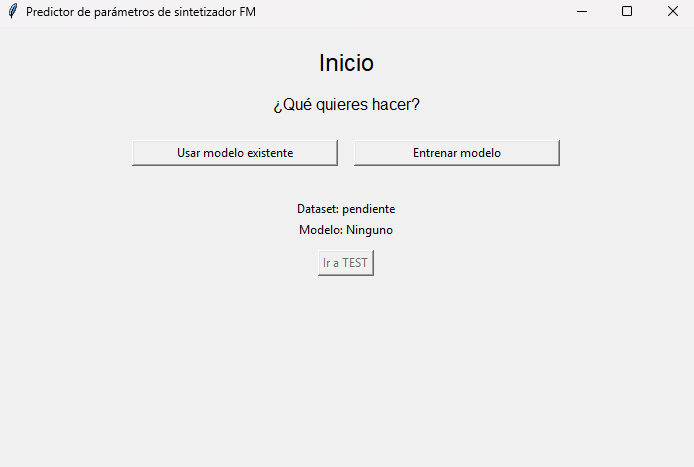
\includegraphics[width=1\textwidth]{Imagenes/Bitmap/pantalla1}
    \caption{Primera pantalla de la Interfaz Gráfica de la Aplicación, elección uso modelo o entrenamiento.}
    \label{fig:pantalla1}
\end{figure}

\begin{figure} 
    \centering
    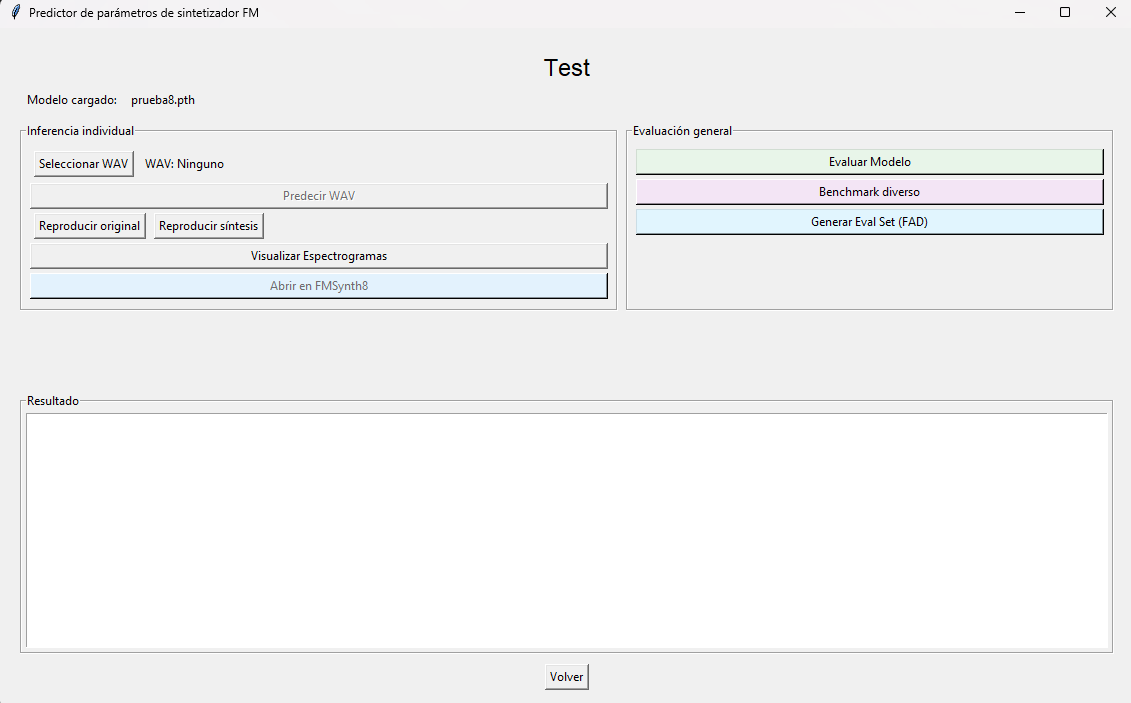
\includegraphics[width=1\textwidth]{Imagenes/Bitmap/pantallaPruebas}
    \caption{Pantalla en la que se pueden hacer pruebas con el modelo seleccionado.}
    \label{fig:pantallaPruebas}
\end{figure}

\begin{figure} 
    \centering
    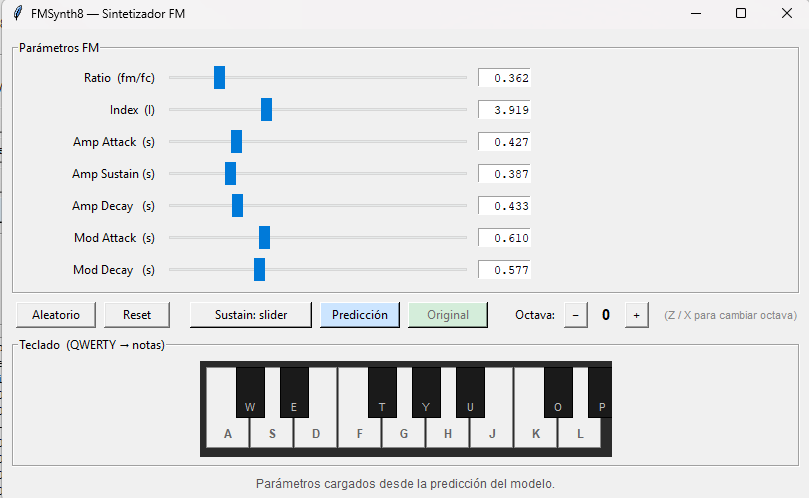
\includegraphics[width=1\textwidth]{Imagenes/Bitmap/sinte}
    \caption{Sintetizador FM de prueba.}
    \label{fig:sinte}
\end{figure}

\begin{figure} 
    \centering
    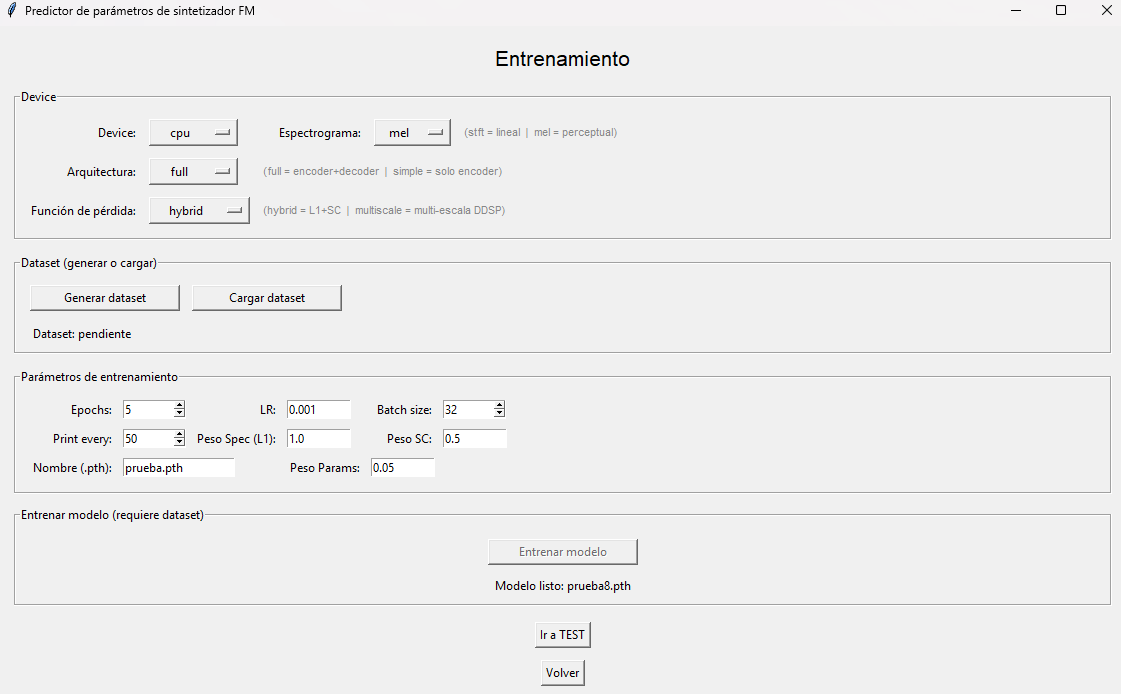
\includegraphics[width=1\textwidth]{Imagenes/Bitmap/pantallaEntrenamiento}
    \caption{Sintetizador FM de prueba.}
    \label{fig:pantallaEntrenamiento}
\end{figure}